\subsection{Forsiden}
\label{sub:Welcome}

Forsidemodulet har til formål at præsentere programmet for brugeren efter log ind.

\subsubsection{Implementation}
\label{ssub:Welcome_implementation}
Forsidemodulet åbnes fra styringsmoduler og er den første fane der vises. Denne fane er tiltænkt til at indeholde genveje med relevans for den bruger, der er logget ind. Derudover vil dette også være et oplagt sted, at have en opslagstavle, med  information fra havnefogeden eller bestyrelsen. Forsiden er med vilje konstrueret simpelt, for at opnå en neutral start. Alternativt kunne en mere funktionel fane, vælges af den individuelle bruger, til at fremstå som deres egen forside.


\begin{figure}
  \centering
  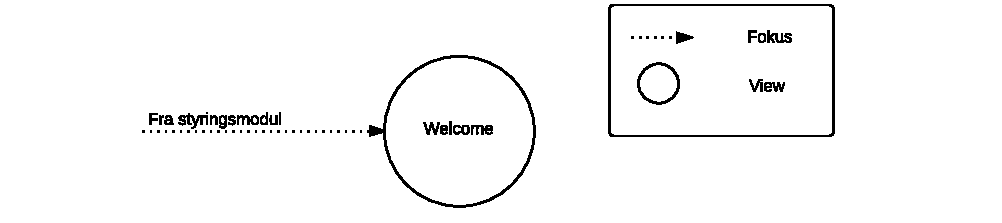
\includegraphics[width=\textwidth]{forside-diagram.pdf}
  \caption{Diagram over forsidemodulet}
  \label{fig:forsidemod}
\end{figure}
